\documentclass{beamer}
\usetheme{Berlin}
\usecolortheme{beaver}

\usepackage{soul}
\sethlcolor{yellow}
\usepackage{graphicx, wrapfig, subcaption}
\usepackage{amsmath, amsfonts, amssymb, amsthm}
\usepackage{upgreek}
\usepackage{mathtools}
%\usepackage[skip=8pt]{parskip}
\usepackage{xcolor, hyperref}
%\usepackage{xspace}
\usepackage{xargs}
%\usepackage[label=\arabic*]{enumitem}
%\usepackage{booktabs}
\usepackage{tabularx}

\usepackage[
    backend=biber
]{biblatex}
\addbibresource{ref.bib}
\usepackage{appendix}

\usepackage{boimacros}

\title{Sinusoidal Distribution}
\subtitle{A new flexible 4-parameter absolutely-continuous probability distribution}
\author{Baidurya Bhattacharyya\inst{1}}
\institute[ISI]{\inst{1} MD2403, M. Stat. 2nd Year\\ Indian Statistical Institute, Kolkata}
\date{\today}

\AtBeginSection[]
{
	\begin{frame}{Contents}
		\tableofcontents[currentsection]
	\end{frame}
}


\begin{document}
\maketitle
\begin{frame}
	\begin{abstract}
		We introduce the \sindist{}, a flexible 4-parameter location-scale-skewness-kurtosis family of distributions, based on Gilbert's Sine distribution (1893). The mathematical properties of this distribution are studied. Examples of fitting the distribution to various statistical objects are considered to demonstrate the distribution's flexibility. Finally, some future avenues are considered for exploration.
	\end{abstract}
\end{frame}

\section{Introduction}
\begin{frame}{The sinusoidal shape}
The sine function over $[0, \pi]$ has a nice `bell" shape indeed. Let us rescale the argument and deal with $\sin(\pi x)$ over $x \in [0,1]$.
\begin{itemize}
    \item But what about its powers -- $\sin^k(\pi x)$ as $k$ varies?
    \begin{figure}
        \centering
        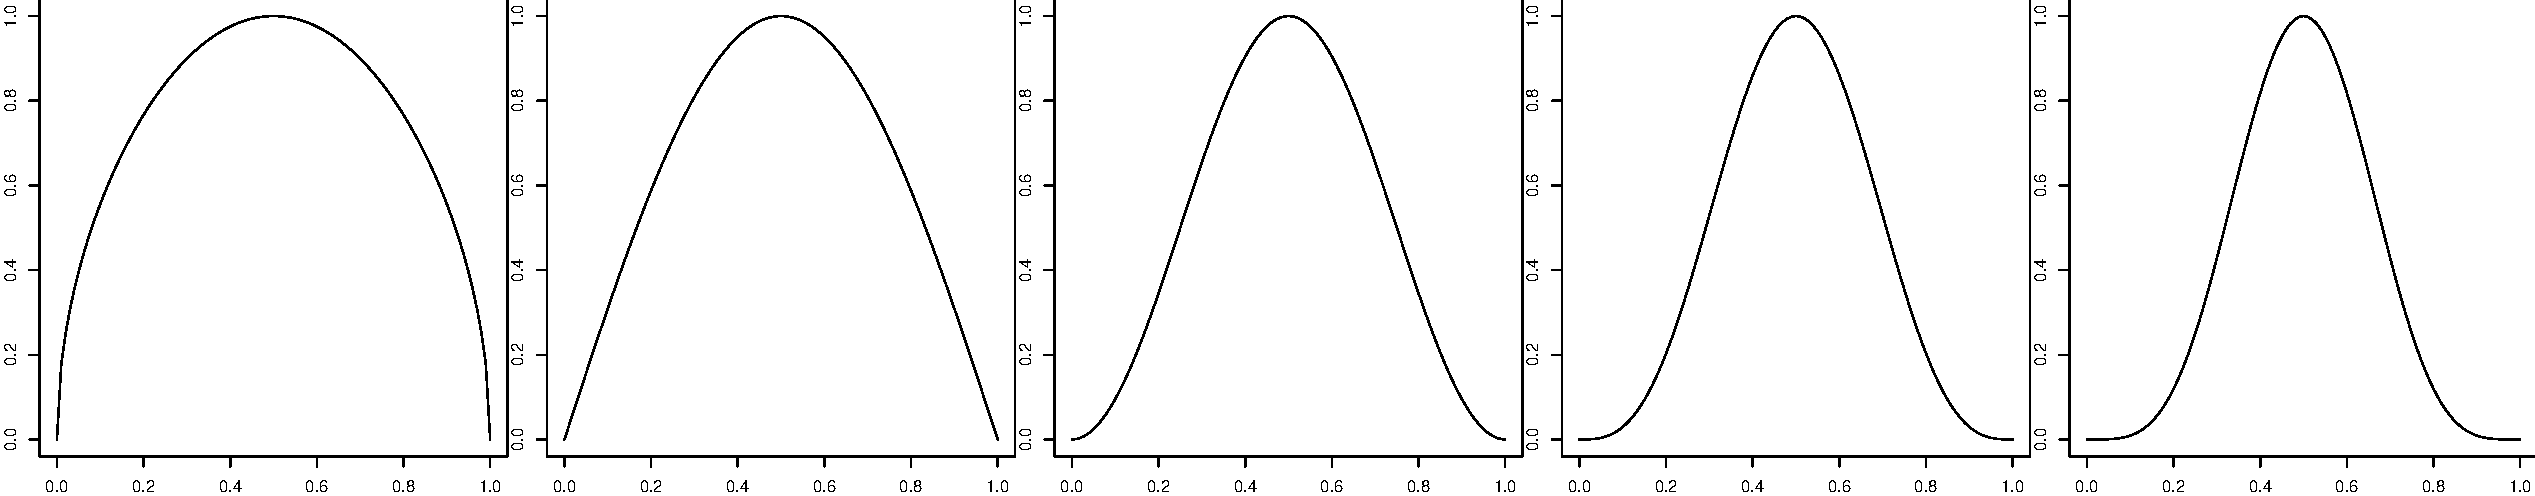
\includegraphics[width=0.5\linewidth]{fig/p1-sinek}
    \end{figure}
    \item And what about powers of its argument -- $\sin(\pi x^s)$ as $s$ varies?
    \begin{figure}
        \centering
        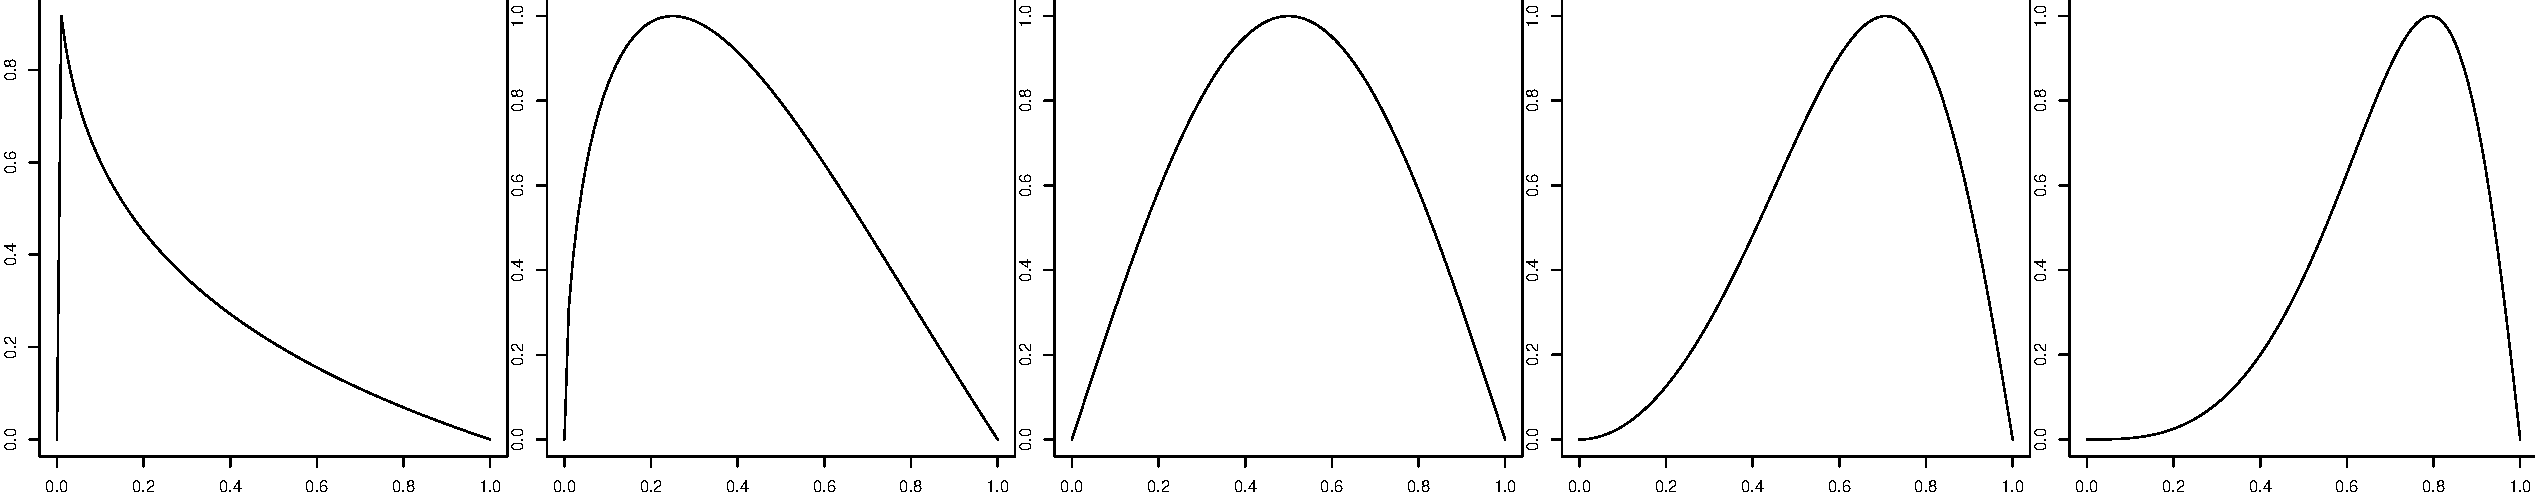
\includegraphics[width=0.5\linewidth]{fig/p1-sines}
    \end{figure}
\end{itemize}
A first attempt at controlling ``peakedness" and ``inclination" intuitively! We can even combine both the operations to control them simultaneously!

\begin{enumerate} \item Hence the choice $\sin^k(\pi z^s)$ for the kernel! \end{enumerate}
\end{frame}

\begin{frame}{Other ``sine" distributions}
    \begin{table}[h]
        \centering
        \begin{tabularx}{\textwidth}{X|X}
            \bfseries Work & \bfseries Distribution \\
            \hline
            \hl{Sine Distribution}, \cite{gilbert1893moon} & $f(z) = \frac{\pi}{2} \sin(\pi z)$ \\
            Sine-G family, \cite{kumar2015bladder} & $F(x) = \sin \left(\frac{\pi}{2} G(x) \right)$ \\
            Transmuted Sine-G family, \cite{sakthivel2021transmuted} & $F(x) = (1+\lambda)\sin \left[\frac{\pi}{2} H(x)\right] - \lambda \sin^2 \left[\frac{\pi}{2}H(x)\right]$\\
            New Sine family, \cite{benchiha2023newsineg} & $F(x) = \frac{\sin \left[\frac{\pi \alpha}{2} G(x)\right]}{\sin \pfrac{\pi \alpha}{2}}$ \\
            Sine generalized-G family, \cite{oramulu2024sinegen} & $F(x) = \sin \left[\frac{\pi}{2} {1-G^\alpha(x)}\right]$\\
            New Transformed Sine-G family, \cite{osi2025ntsg} & $F(x) = \frac{\exp \sin \bfrac{\pi H(x)}{1+h(x)} - 1}{\e - 1}$\\
            Sine-Frechet-G family, \cite{jerry2026frechet} & $F(x) = \sin \left[\frac \pi 2 \exp{-b^a (-\ln{1-G(x)})^{-a}}\right]$
        \end{tabularx}
        \caption{Existing distributions involving the sine function}
        \label{tab:othersines}
    \end{table}
\end{frame}

\section{The Distribution}
\begin{frame}{Standard Sinusoidal Distribution}
Notation: $Z \sim \Sinu(s,k)$
\begin{enumerate}
    \item Parameters: $s \ge 0$, $k\ge 0$
    \item Kernel: $\varsigma(z; s,k) := \sin^k(\pi z^s)$
    \item Normalizing constant $A(s,k) := \int_0^1 \sin^k(\pi t^s) \d t$
    \item PDF: $\psi(z; s,k) \equiv \frac{\varsigma(z; s,k)}{A(s,k)} = \frac{1}{A(s,k)} \sin^k(\pi z^s); \quad z \in [0,1]$
    \item $\Psi(z; s,k) = \int_0^z \psi(t; s,k) \d t \equiv \frac{A_z(s,k)}{A(s,k)}; \quad z\in[0,1]$ where $A_z(s,k)$ denotes the incomplete integral of the kernel
    
\end{enumerate}
\end{frame}

\begin{frame}{Plots}
   \begin{figure}
        \begin{subfigure}{0.45\textheight}
            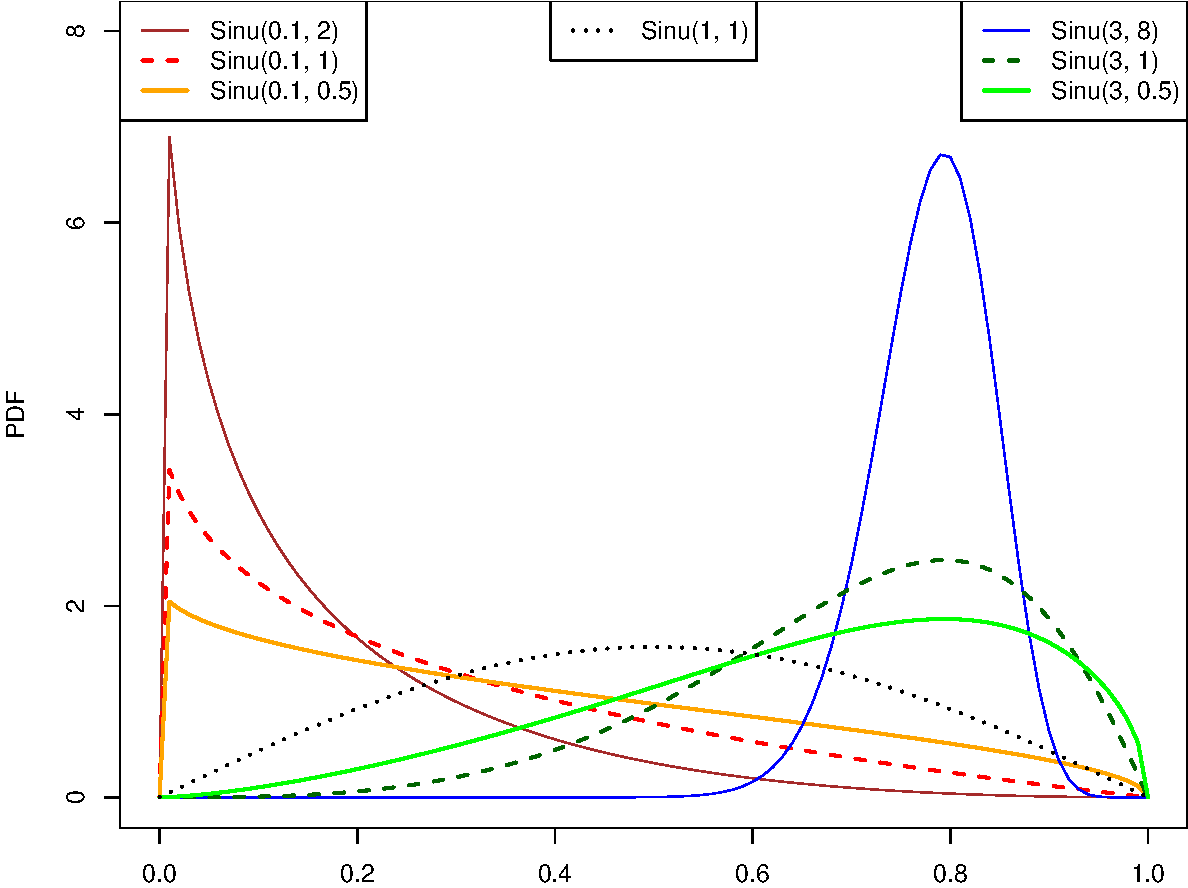
\includegraphics[width=\linewidth]{fig/2-pdf}
            \caption{PDFs}
        \end{subfigure}
        \begin{subfigure}{0.45\textheight}
            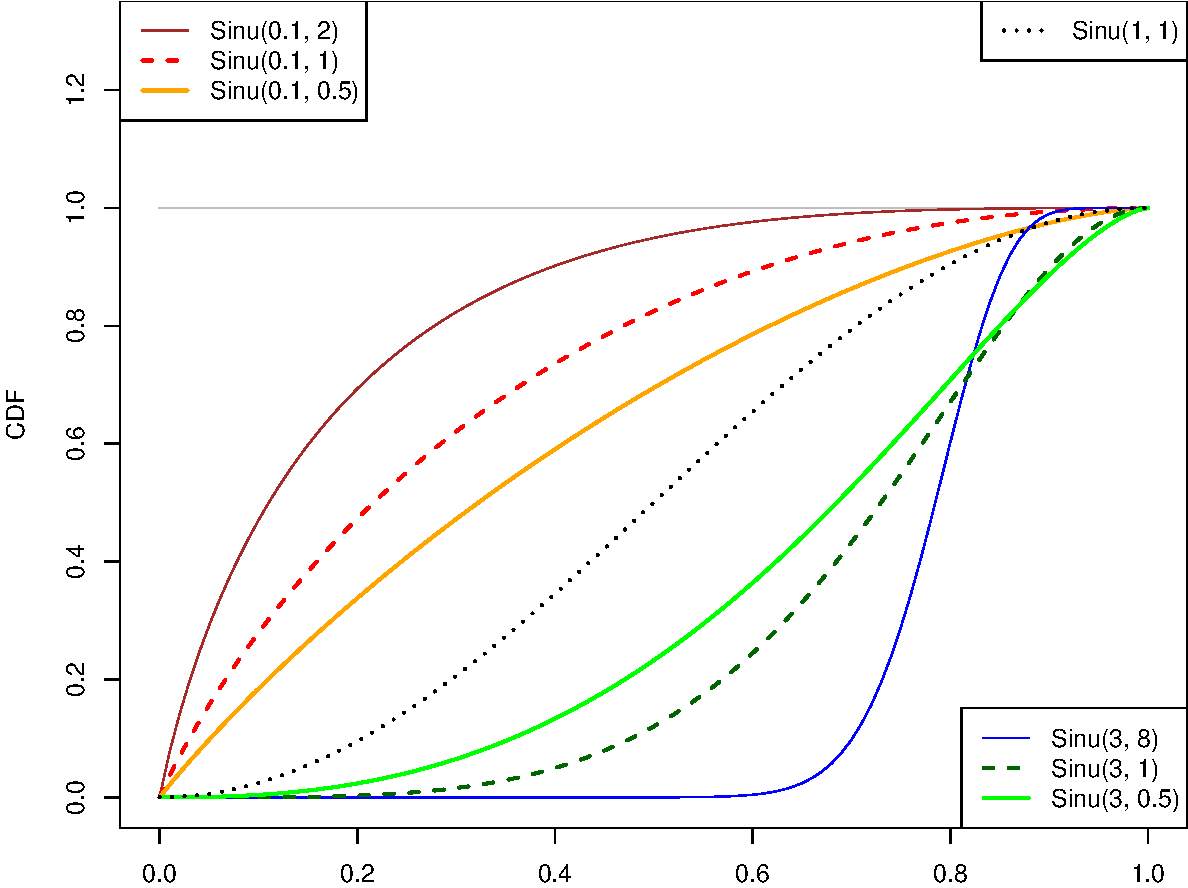
\includegraphics[width=\linewidth]{fig/2-cdf}
            \caption{CDFs}
        \end{subfigure}
        \begin{subfigure}{0.45\textheight}
            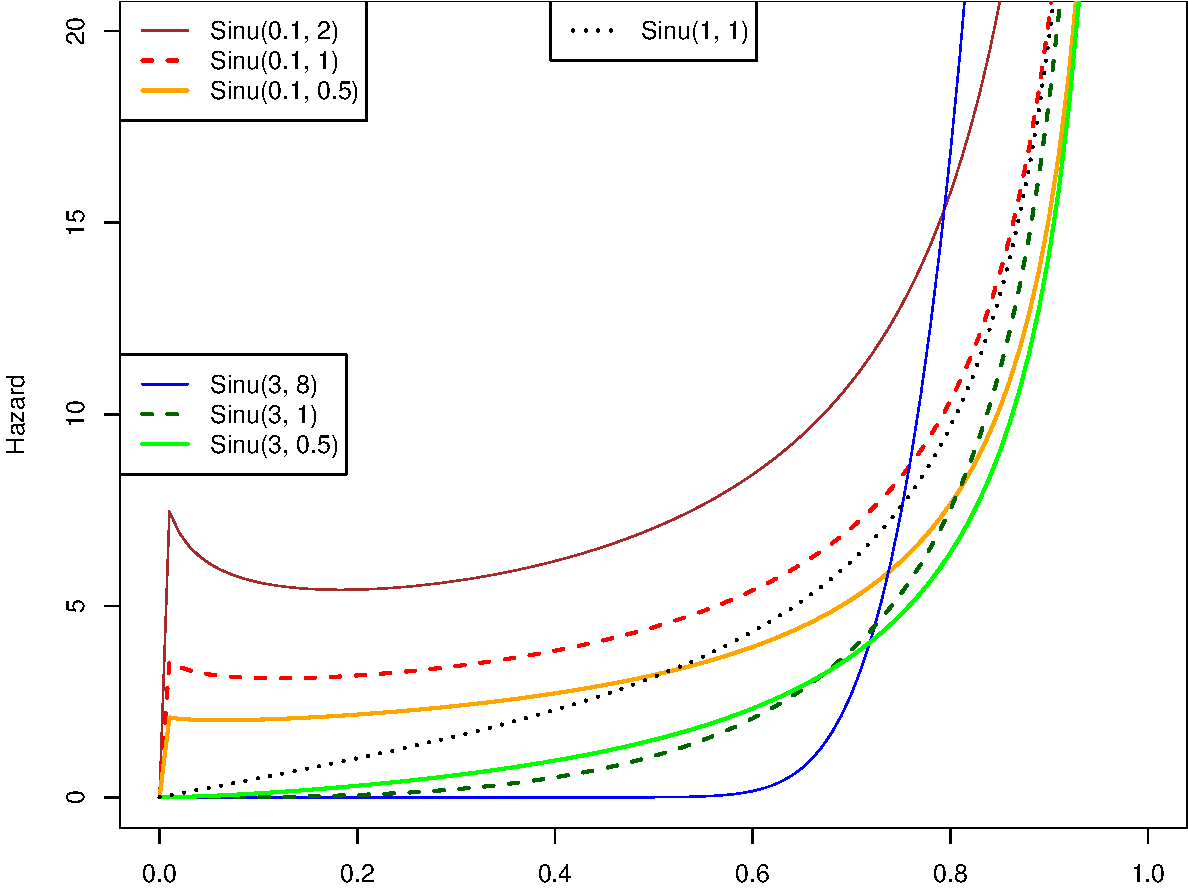
\includegraphics[width=\linewidth]{fig/2-hf}
            \caption{Hazard Functions}
        \end{subfigure}
        \begin{subfigure}{0.45\textheight}
            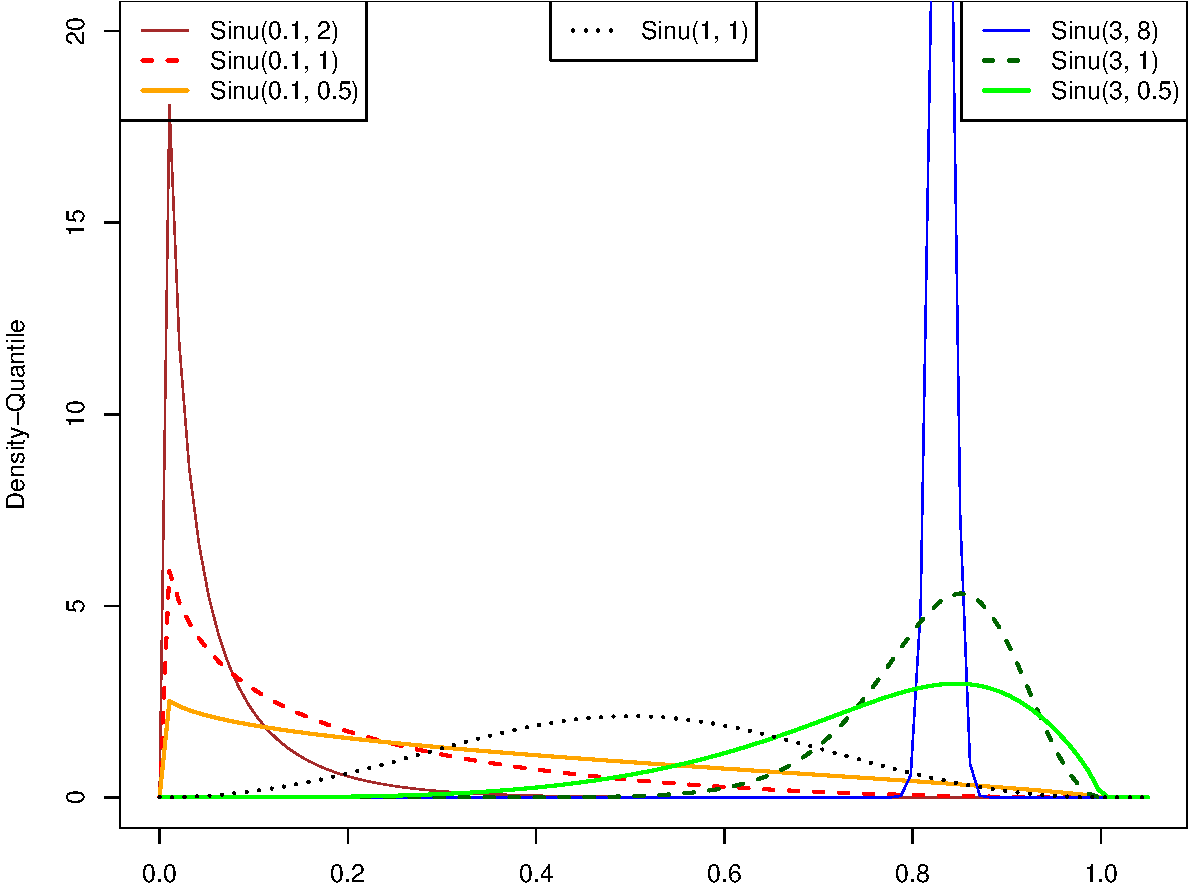
\includegraphics[width=\linewidth]{fig/2-dqf}
            \caption{DQFs}
        \end{subfigure}
        \caption{Shape plots of different \sindist s}\label{fig:shapeplots}
    \end{figure}
\end{frame}

\begin{frame}{Extensions}
\begin{enumerate}
    \item Location-Scale extension: $\psi(x; a,d,s,k) = {\frac 1 d} \psi \left( \frac{x-a}{d}; s,k \right);  \quad x \in [a, a+d]$ with parameters $a \in \RR, d \ge 0, s \ge 0, k\ge 0$
    \item Flipped extension: $ \pi'(x; a,d,s,k) = {\frac 1 d} \psi \left( \frac{a+d-x}{d}; s,k \right)$
\end{enumerate}
\end{frame}

\begin{frame}{Shape properties}
\begin{enumerate}
    \item Parameters: Location: $a \in \RR$, $d\ge0$, $s\ge0$, $k\ge0$
    \item Support $[a,a+d]$
    \item $s=1$: symmetric. Left and right tilts on respective sides of equality.
    \item Increasing $k$ first increases but then decreases kurtosis
    \item Mode: $2^{-1/s}$, Modal density: $1/A(s,k)$
\end{enumerate}
\end{frame}

\begin{frame}{Skewness-Kurtosis Interdependence on $s,k$}
\begin{figure}
    \begin{subfigure}{0.48\linewidth}
        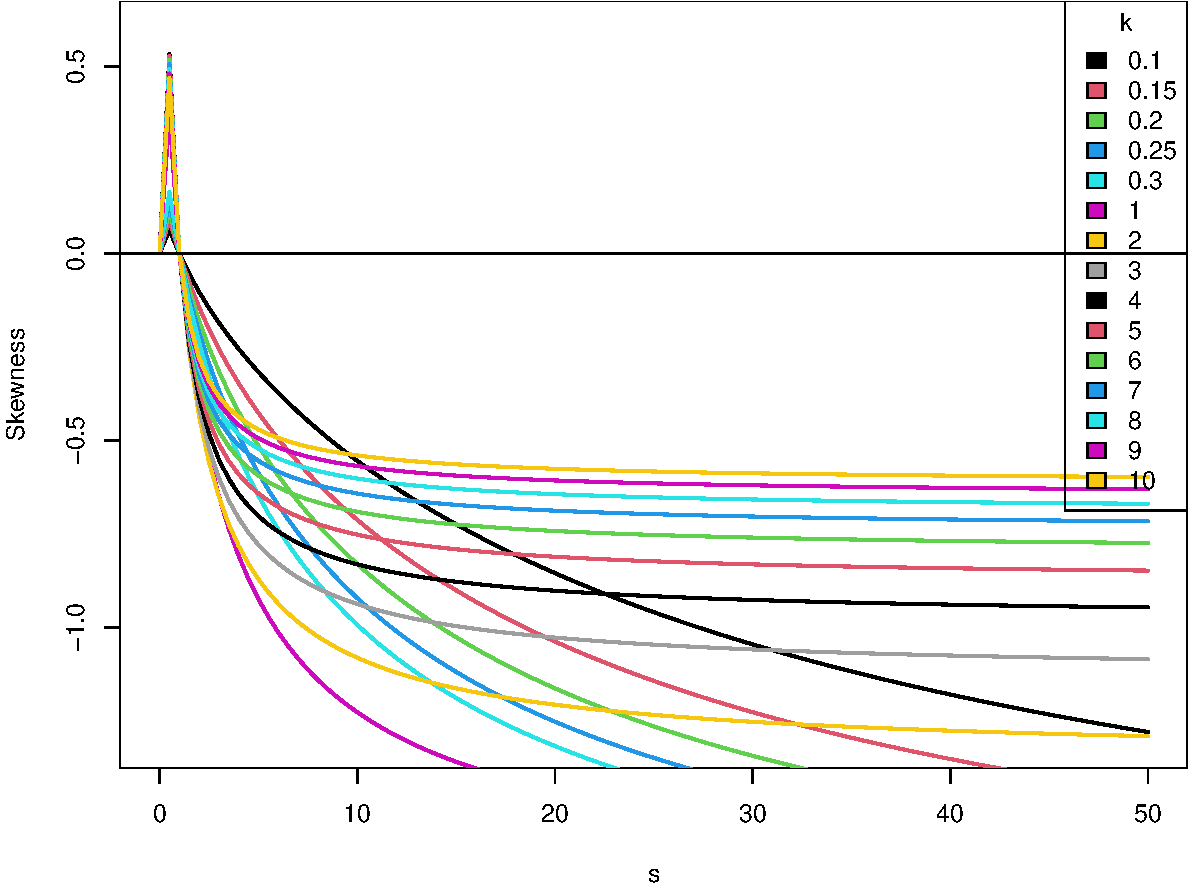
\includegraphics[width=\linewidth]{fig/2-skewvss}
        \caption{Skewness vs. $s$}
    \end{subfigure}
    \begin{subfigure}{0.48\linewidth}
        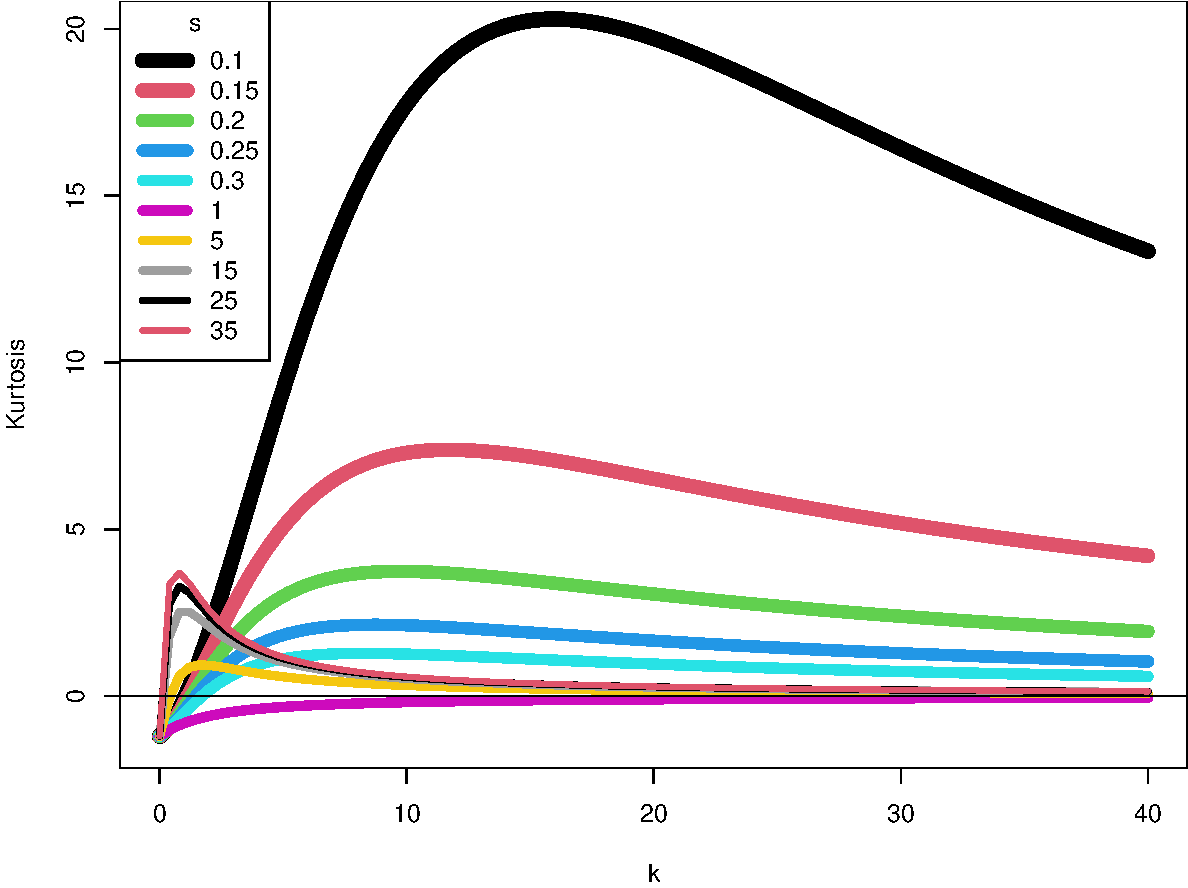
\includegraphics[width=\linewidth]{fig/2-kurtvsk}
        \caption{Kurtosis vs. $k$}
    \end{subfigure}
    \caption{$s$, $k$ jointly affect skewness \& kurtosis}\label{fig:skassoc}
\end{figure}
\end{frame}


\section{Mathematical Properties}
\begin{frame}[allowframebreaks, allowdisplaybreaks]{Mathematical Properties}
\begin{enumerate}
	\footnotesize
    \item $\Sinu(s,k)$ distribution corresponds to the intensity of crater activity on the planetary surface given by the radial curve $r(z) = r_0 \exp\left(\int_0^{\pi z^s} \tan(t - \sin^{-1}\sin^k t) \d t\right)$
    \item $X_1, \dots, X_n \iidsim \Sinu(a,d,s,k)$ have joint density $f(x_1\dots x_n) = \frac{1}{A^n(s,k) 2^{nk} d^n } \left( \sum_{r_1=\pm1}\cdots \sum_{r_n = \pm 1} \left[\prod_{j=1}^n r_j\right] \cdot \exp\left[\sum_{j=0}^n \i \pi r_j \left(\frac{x_j -a}{d}\right)^s\right]  \right)^k$
    \item $\Sinu(a,d,s,k)$ is sub-Gaussian with parameter $d^2/4$
    \framebreak \scriptsize
    \item The normalizing constant for the symmetric case is $A(1,k) = \frac{2^k}{\pi} \frac{\Gamma^2\left( \frac{k+1}{2} \right)}{\Gamma\left( k+1\right)} \equiv \frac{1}{\sqrt \pi} \frac{\Gamma\left(\frac{k+1}{2}\right)}{\Gamma\left(\frac{k}{2} + 1\right)}$
    \item Incomplete integral of the symmetric ($s=1$) kernel for $k\in \ZZ^+$ is given as:
        \begin{align}
    	\int_0^z \sin^k\pi t \, dt =
    	\frac{1}{2^{2n}} {2n \choose n} z + \frac{(-1)^n}{\pi 2^{2n-1}}\sum_{k=0}^{n-1} (-1)^k {2n \choose k} \frac{\sin 2(n-k)\pi z}{2(n-k)} && [\text{$k=2n$}]\\
    	= \frac{1}{\pi 2^{2n}}(-1)^n \sum_{k=0}^n (-1)^k {2n+1 \choose k} \frac{1 - \cos (2n+1-2k)\pi z}{2n+1-2k}  &&  [\text{$k=2n+1$}]
    	\end{align}
    \item Taking $d = \pi \sqrt k$ and letting $k \to \infty$, a symmetric about 0 Sinusoidal density, $\Sinu\left(-\frac d 2, d, 1, k\right)$ tends to a Standard Normal density;  i.e. $\psi_k(x) \to \phi(x)$ as $k \uparrow\infty$
\end{enumerate}
\end{frame}

\begin{frame}{Tending normality}
	\begin{figure}
		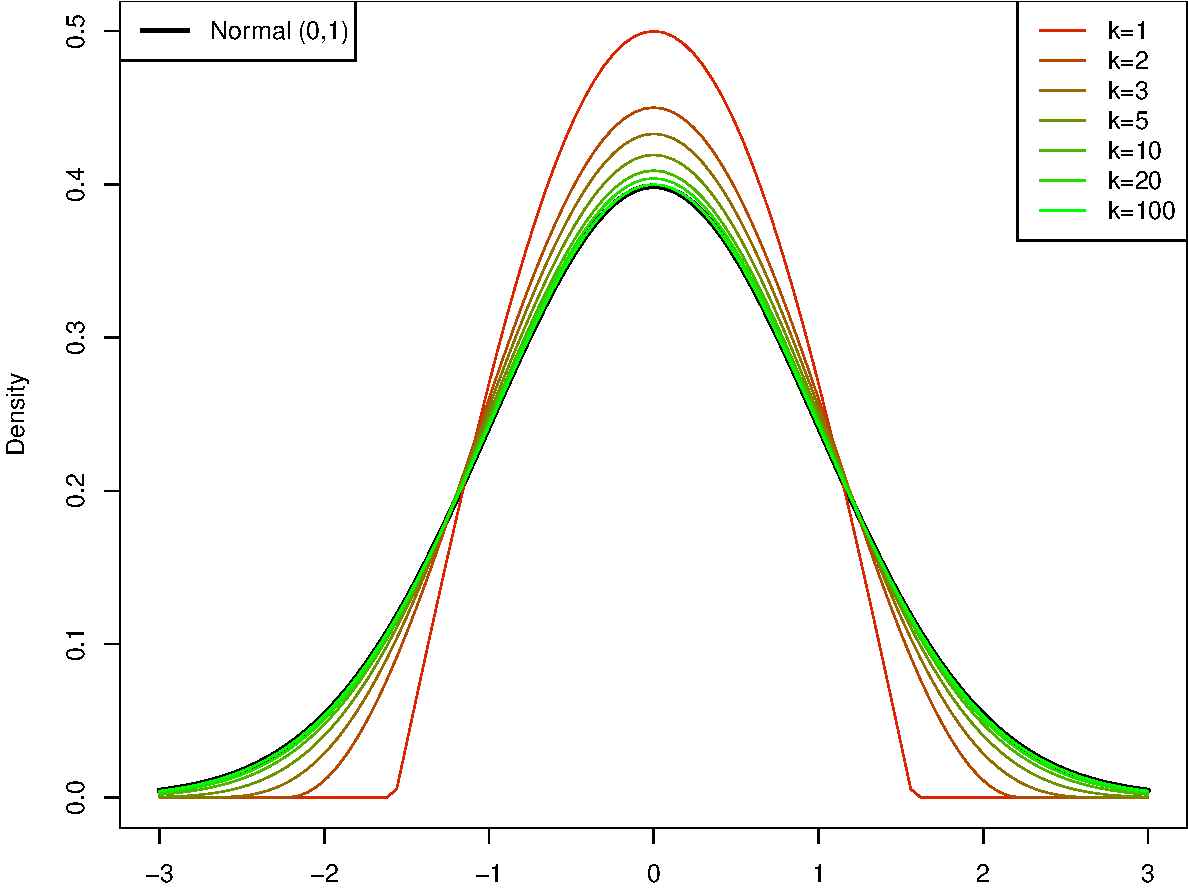
\includegraphics[height=0.7\textheight]{fig/2-tendingnormal}
		\caption{Sinusoidal distributions tending closer to $\N (0,1)$ as $k \uparrow \infty$}
	\end{figure}
\end{frame}

\section{GHGF}

\begin{frame}{Context}
	\begin{enumerate}
		\item A distribution family without explicit formulae for its CDF, moments, MGF, CF, etc. misses its true potential
		\item No matter how flexible, it is difficult to work with on paper
		\item Chances are that such a distribution is also a computational nightmare during fitting, inference, etc.
		
	\end{enumerate}
\end{frame}

\begin{frame}{Introducing the GHGF}
	\textbf{Generalized Hypergeometric Function (GHGF)} $\Fhyp_q^p$, parametrized by $a_1, \dots, a_p$ and $b_1, \dots, b_p$, calculated at the argument $x$ is: 
	\[\Fhyp_q^p \left(\begin{matrix} a_1 & \cdots & a_p \\ b_1 & \cdots & b_q\ \end{matrix} ; x \right) := \sum_{j=0}^\infty \frac{\poch{a_1}[j] \cdots \poch{a_p}[j]}{\poch{b_1}[j] \cdots \poch{b_q}[j]} \frac{x^j}{j!}\]
	where $\poch x := x(x+1)\cdots(x+n-1)$ is the \textbf{rising factorial / Pochhammer function}.
	
	Also denote ${r \choose k} = \frac{\poch{r}[k]}{k!}$ as the \textbf{generalized Binomial coefficient}.
\end{frame}

\begin{frame}[allowframebreaks]{Strategies}
	Depending on the purpose and the form of the function at hand, the following strategies may work into providing simple explicit expressions for the statistical properties of the \sindist:
	\begin{enumerate}
		\item Euler expansion: $\sin \theta = \frac{\e^{\i\theta}-\e^{-\i\theta}}{2\i}$
		\item Maclaurin series expansion only when exponents are not involved; otherwise complicated ``generalized Multinomial expansion" viz. $\sin^k(x) = \left(x - \frac{x^3}{3!} + \frac{x^5}{5!}- \cdots \right)^k$, which quickly becomes intractable.
		\item Identifying a GHGF upto a scalar multiple from its ratio of terms, since $\frac{\Fhyp_{n+1}}{\Fhyp_n} \left[ \begin{matrix} a_1 \cdots a_p \\ b_1 \cdots b_1 \end{matrix}; z \right] = \frac{(a_1 + n) \cdots (a_p +n)}{(b_1 +n)\cdots(b_q +n)} \frac{z}{n+1}$
	\end{enumerate}
\end{frame}

\begin{frame}[allowframebreaks]{Properties}
All properties below are described for the Standard \sindist{} $\Sinu(s,k)$. Location-scale families can be easily extended to.
	\begin{enumerate}
		\item The kernel $\sin^k (\pi z^s)$ can be given as
		$(\pi z^s)^k \left( \Fhyp^0_1 \left[ \begin{matrix} \cdot \\ \frac{3}{2} \end{matrix}; -\frac{\pi^2 u^2}{4}\right] \right)^k$, or using the GHGF as $\Fhyp^1_0 \left[ \begin{matrix}k\\ \cdot\end{matrix};  -\exp(-2 \i \pi z^s) \right]$.
		\item The characteristic function can be given as $\frac{1}{A(s,k) (2\i)^k} \sum_{j=0}^{\infty} (-1)^j \binom{k}{j} \sum_{m=0}^{\infty} \frac{(\i t)^m}{(m+1)!} \Fhyp^1_1\left[ \begin{matrix}\frac{m+1}{s}\\ \frac{m+1}{s} + 1 \end{matrix};\, \i\pi(k-2j) \right]$.
		\item Thus the MGF becomes $\frac{1}{A(s,k) (2\i)^k} \sum_{j=0}^{\infty} (-1)^j \binom{k}{j} \sum_{m=0}^{\infty} \frac{t^m}{(m+1)!} \Fhyp^1_1\left[ \begin{matrix}\frac{m+1}{s}\\ \frac{m+1}{s} + 1 \end{matrix};\, \i\pi(k-2j) \right]$
		\item The expression for the $r$\textsuperscript{th} order moment is $\upmu_r(s,k) = \frac{1}{A(s,k) (2\i)^k (r+1)} \sum_{j=0}^{\infty} (-1)^j \binom{k}{j} \Fhyp^1_1 \left[ \begin{matrix}\frac{r+1}{s} \frac{r+1}{s} + 1\end{matrix}; \, \i\pi(k-2j) \right]
		= \frac{1}{A(s,k) (2\i)^k} \sum_{j=0}^\infty {k \choose j} (-1)^j \sum_{n=0}^{\infty} \frac{[\i (k-2j) \pi]^n}{n! (ns+r+1)}$
		\item CDF is given by $ \Psi(z; s,k) = \frac{1}{A(s,k) (2\i)^k} \sum_{j=0}^\infty (-1)^j {k \choose j} \sum_{n=0}^{\infty} \frac{[\i (k-2j) \pi]^n}{n! (ns+1)} z^{ns+1}$
		\item The normalizing constant is given by $\frac{1}{(2\i)^k} \sum_{j=0}^\infty (-1)^j {k \choose j} \sum_{n=0}^{\infty} \frac{[\i (k-2j) \pi]^n}{n! (ns+1)}$
	\end{enumerate}
\end{frame}

\section{Fitting}
\begin{frame}{Fitting Methods}
	The following routes for fitting the \sindist{} have been thought of:
	\begin{enumerate}
		\item MLE on sample observations
		\item MSM on MSM
		\item PDF on PDF
		\item CDF on CDF
		\item CDF on ECDF
	\end{enumerate}
	Currently, (3) has been briefly implemented and (1), (2) discussed.
\end{frame}

\begin{frame}[allowframebreaks]{MLE on Data}
	Joint likelihood:
	\[ l(a,d,s,k; \utilde x)
	= -n\ln(d)-n\ln(A(s,k)) + k\sum_{i=1}^n \ln \sin \pi\left( x_i-a \over d \right)^s\]
	Calculating the preliminary derivatives:
	\begin{align*}
		\nabla_s A &= \pi k \int_0^1 \sin^{k-1}(\pi z^s) \cos(\pi z^s) (\ln z) z^s \ \d z\\
		\nabla_k A &= \int_0^1 \sin^k(\pi z^s) \ln \sin(\pi z^s) \ \d z
	\end{align*}
	Gives us the following score equations:
	\begin{align*}
		\nabla_a \ell = 0 &\iff \sum_{i=1}^n z_i^{s-1} \cot(\pi z_i^s) = 0\\
		\nabla_d \ell = 0 &\iff \pi sk \sum_{i=1}^n z_i^s \cot(\pi z_i^s) = -n \\
		\nabla_s \ell = 0 &\iff  \pi k \sum_{i=1}^n {z^s \cos \pi z^s \ln z  \over \sin \pi z^s} = n {\nabla_s A \over A}\\
		\nabla_k \ell = 0 &\iff \sum_{i=1}^n \ln \sin \pi z_i^s = n{\nabla_k A \over A}
	\end{align*}
	\begin{itemize}
		\item Difficult to simultaneously solve
		\item Computational maximization may be considered
	\end{itemize}
\end{frame}


\begin{frame}{MSM on MSM}
	\scriptsize
	The skewness-kurtosis cover-plot of $\Sinu(s,k)$ for the parameter range $s,k \in 0.5 \, (0.5)\, 6$:
	\begin{figure}[h]
		\centering
		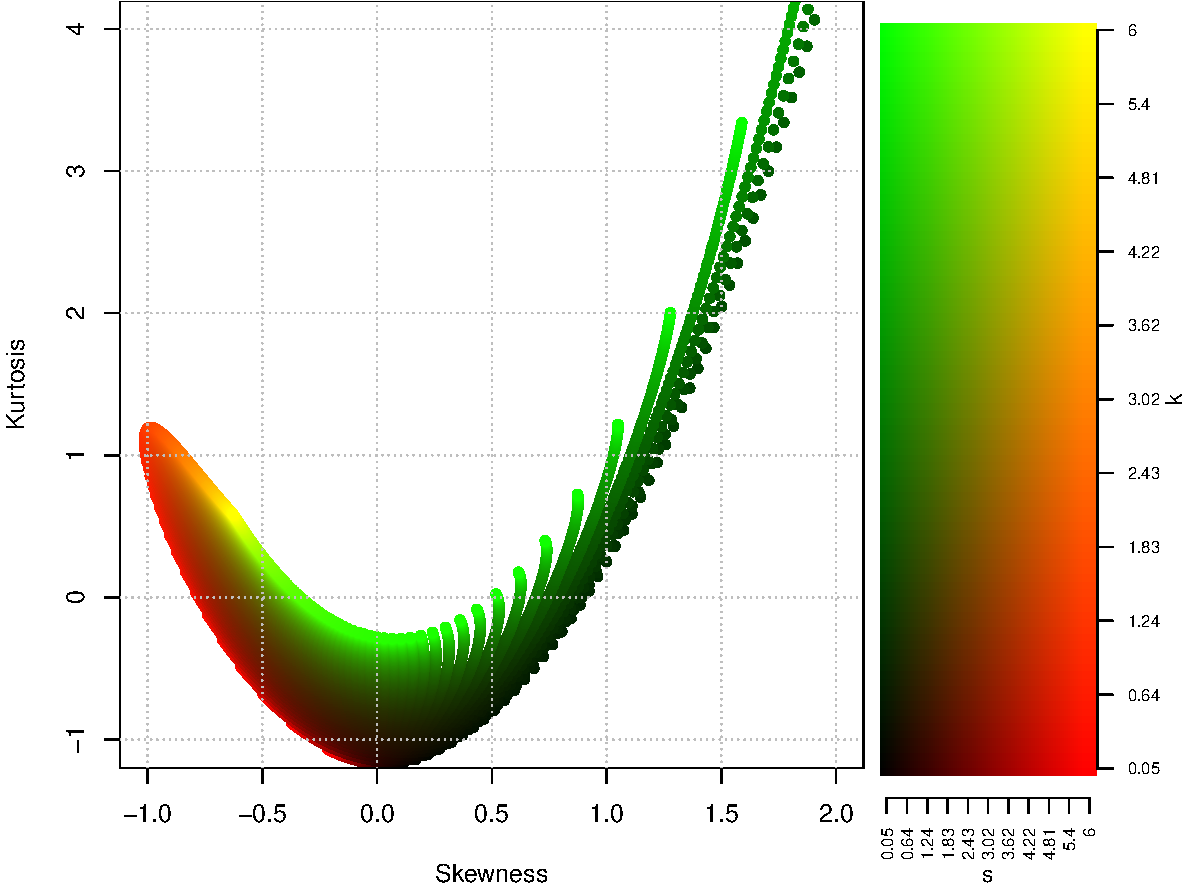
\includegraphics[width=0.6\linewidth]{fig/2-skewkurtcover}
	\end{figure}
	Choice of loss function and optimization methods will be considered in the next iteration.
\end{frame}

\begin{frame}[allowframebreaks]{PDF on PDF}
	\begin{enumerate}
		\item $g(x)$: target density, $f \equiv \psi(x;a,d,s,k)$: candidate density.
		\item Hellinger loss function: $L(a,d,s,k) = 1 - \int \sqrt{\psi(x;a,d,s,k)g(x)} \d x$
		\item Parameter range for computational finiteness:  $a \in [-10^3, 10^3]$, $d \in [10^{-2}, \, 2\times10^3]$, $s \in [10^{-2}, 10^2]$ and $k \in [10^{-2}, 10^2]$.
		\item \texttt{R}'s \texttt{optim} function, \texttt{L-BFGS-B} method used to optimize the loss function.
	\end{enumerate}
	
	\scriptsize
	\begin{table}
		\centering
		\begin{tabularx}{\linewidth}{c|X}
			Target Density & Hellinger distance (Choice of Parameters $a,d,s,k$)\\
			\hline
			$\N(0,1)$ & 0.00004277289 (-20.542932, 34.985498, 1.304535, 100)\\
			$\mathrm{Lognormal}(0,1)$ & 0.000936801 (0.02827762, 1000, 0.08566970, 35.78972) \\
			$\mathrm{Skew}\N_{\alpha=1} (0,1)$ & 2.189446e-05 (-7.2216216, 24.8516728, 0.5936823, 100) \\
			\hline
			$\mathrm{Logistic}(0,1)$ & 0.003149183 (-80.275639, 102.222513, 2.882431, 100) \\
			$\mathrm{Exp}(1)$ & 0.008101119 (0.0005708485, 6.5585684475, 0.0621246472, 1.6766166256) \\
			$\mathrm{DE}(0,1)$ & 0.01599712 (-8.895071, 16.872288, 1.085768, 15.608238) \\
			\hline
			$\Gamma(0.1,1)$ & Poor fit \\
			$\Gamma(100,1)$ & Poor fit \\
			$\Beta(1,1)$ & 0.0030202, (-0.0007780335, 1.0012066335, 0.1004892336, 0.12190192670) \\
			\hline
			$\mathrm{Cauchy}(0,1)$ & 0.06878475 (-126.211809, 149.303341, 4.141315, 100) \\
			\hline
			$\chi^2(1)$ & Poor fit \\
			$\chi^2(10)$ & 5.791378e-06 (-0.3201950, 97.1337699, 0.2815837, 22.0271292) \\
			$\mathrm{t}_1(0,1)$ & 0.06878477 (-126.114092, 149.207078, 4.138119, 100) \\
			$\mathrm{t}_{10}(0,1)$ & Fit failed \\
			$\mathrm{F}(1,1)$ & Poor fit
		\end{tabularx}
	\end{table}
	\begin{figure}
		\centering
		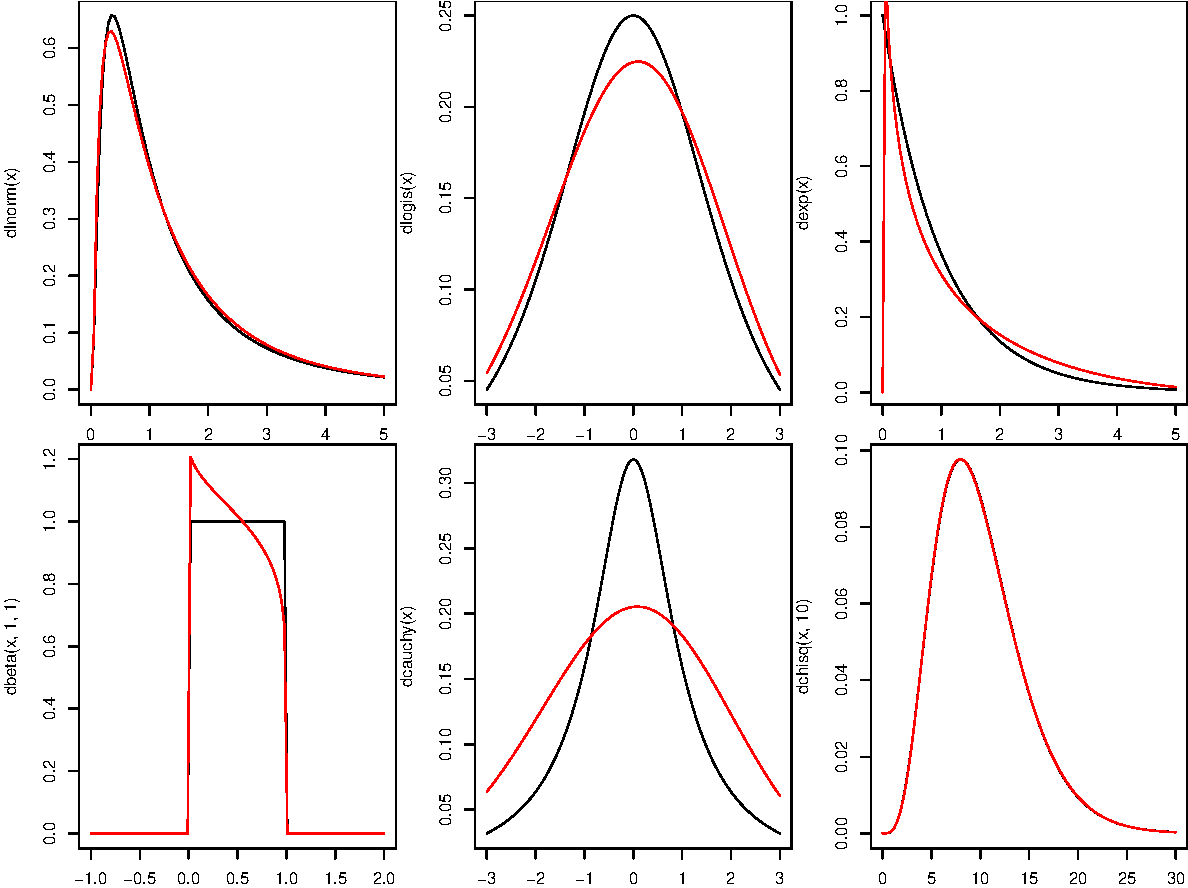
\includegraphics[width=0.7\linewidth]{fig/3-pdfonpdf}
		\caption{Some results from PDF on PDF fitting using above methodology}
	\end{figure}
	\normalsize
	\begin{enumerate}
		\item Results greatly dependent on initialization of parameters
		\item The nature of the Hellinger metric affects the fit. It will be a task to investigate the effect of other metrics on PDF on PDF fitting.
		\item Certain distributions seem to be out of the shape-coverage (at least skewness-kurtosis coverage) of the \sindist.
	\end{enumerate}
\end{frame}

\begin{frame}{CDF on Data (ECDF)}
	We work with the following strategy:
	\begin{enumerate}
		\item Extract $a$ and $a+d$ as \texttt{max(data)} and \texttt{min(data)} respectively
		\item Normalize the data to fall in the $[0,1]$ range
		\item Fit a $\Sinu(0,1,s,k)$ distribution over the 
	\end{enumerate}
\end{frame}

\section{Future Objectives}
\begin{frame}
	\begin{enumerate}
		\item Further investigation and simplification of analytical properties
		\item Investigation of its replication capacity, parametric-limiting nature
		\item Devising fitting algorithms for more pairs of statistical objects, and newer methods for existing ones
		\item Studying the effect of different metrics on fits. Characterization of metrics to some degree
		\item Modelling the distribution of complicated statistics
		\item Fitting to unconventional datasets, especially in survival statistics and econometrics
		\item Usage as flexible Bayesian priors with the further incorporation of variable skewness and kurtosis
		\item Usage as a flexible learnable-multiparameter activation function for NNs. Comparison against existing methods.
	\end{enumerate}
\end{frame}

\frame{Thank You}

\begin{frame}[allowframebreaks]{References}
	\scriptsize \printbibliography
\end{frame}

\end{document}